The output of the data-processing pipeline described in \sref{data} is the data
set $X$, which is split into three parts: $X_1$ is for the training stage, $X_2$
for the validation stage, and $X_3$ for the testing stage. In what follows, we
elaborate on the processes that are taking place during these three stages of
working with the model presented in \sref{model}.

\subsection{Training} \slab{training}
The model in \sref{model} has a large number of parameters that have to be
learned during training; they are primarily various wights and biases inside the
model's layers. For this purpose, $X_1$ is utilized. The training is undertaken
via backpropagation through time using stochastic gradient descent
\cite{goodfellow2016} whose objective is to minimize a certain loss function,
which we shall specify shortly. The variant of gradient descent that we use is
Adam \cite{kingma2014}, which is an adaptive optimization method. There are two
aspects to be discussed about training.

\begin{figure}[t]
  \centering
  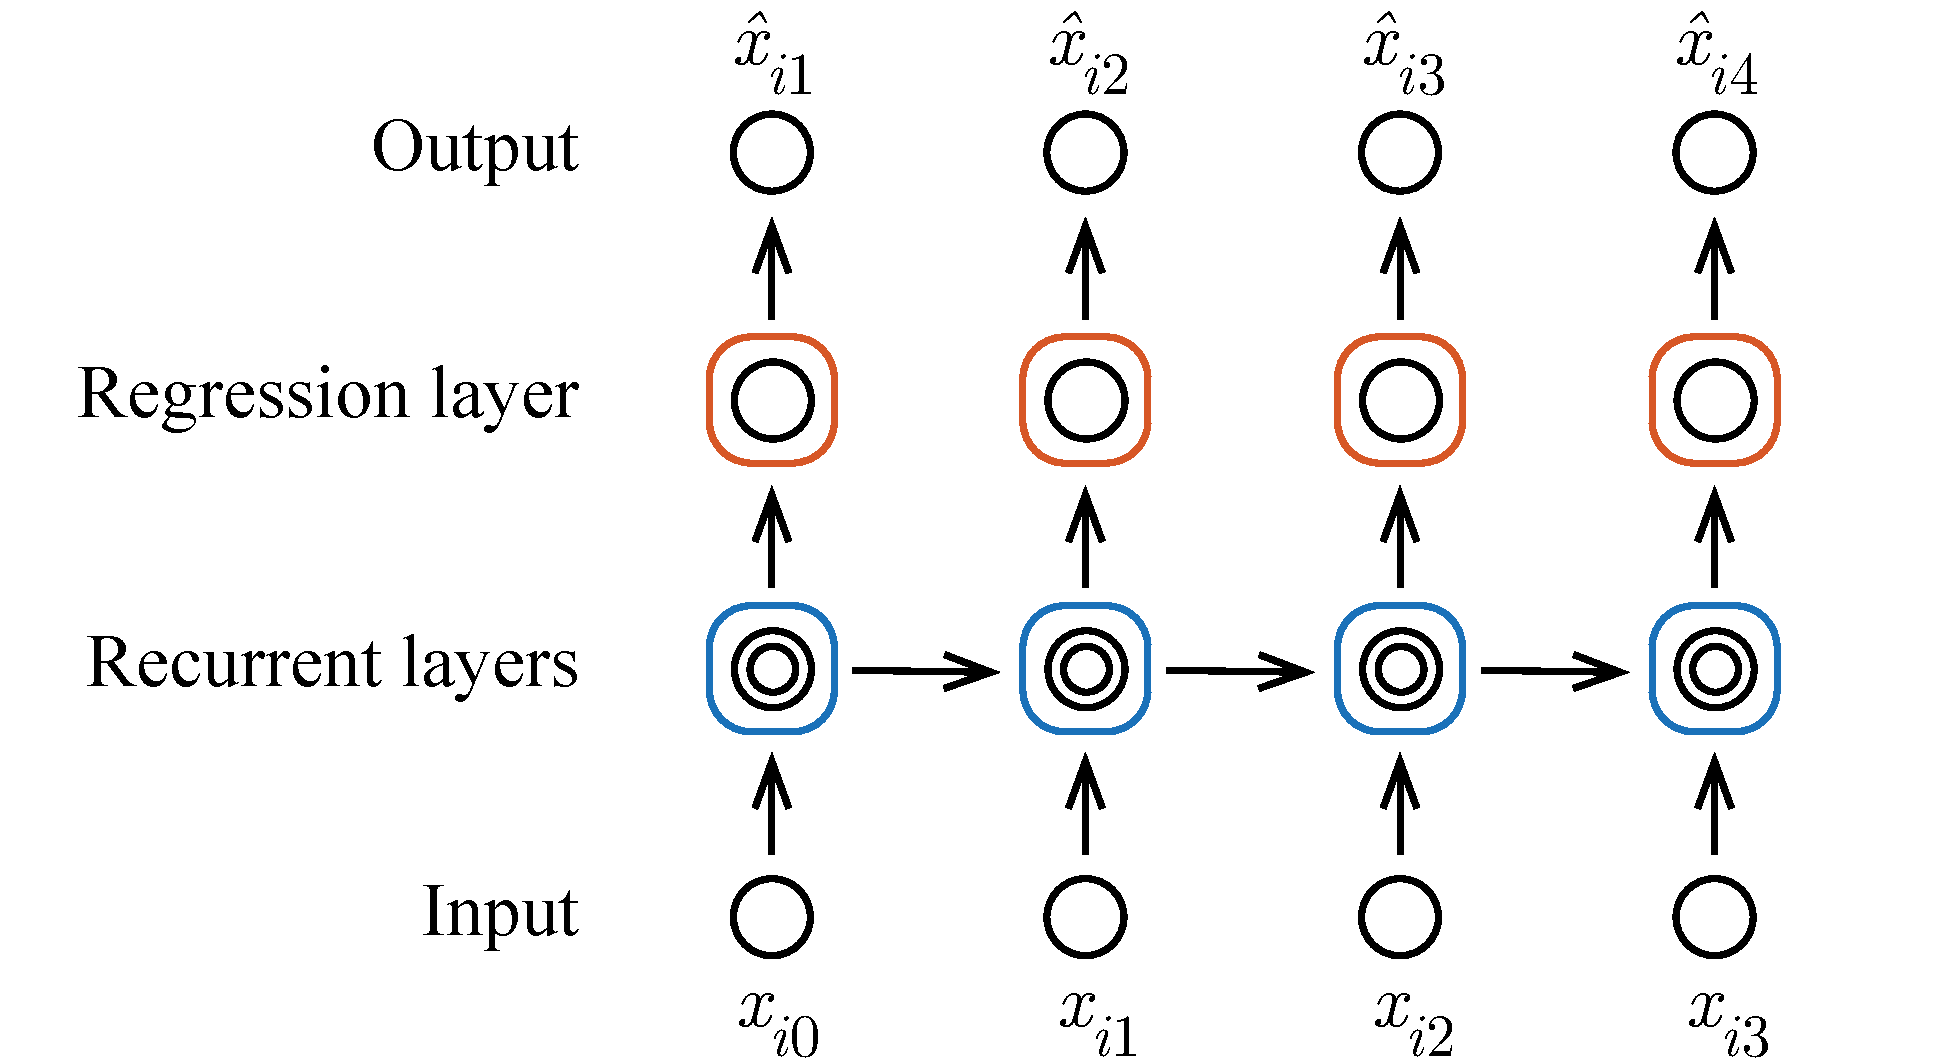
\includegraphics[width=1.0\columnwidth]{include/assets/figures/unroll.pdf}
  \vspace{-2.0em}
  \caption{Example of dynamic unrolling during the model's usage.}
  \vspace{-1.5em}
  \flab{unroll}
\end{figure}

The first concerns the way a single resource-usage trace is fed into the model.
First, note that a trace has multiple data points ($l_i > 1$), and that two
traces are of different lengths in general ($l_i \neq l_j$) since the execution
times of different tasks can differ substantially. All the points of a trace are
fed in one pass using a technique called dynamic unrolling. An illustration for
$l_i = 4$ is given in \fref{unroll}, in which the representation in \fref{model}
has been simplified even further and put on a side. It can be seen that the
model has been replicated as many times are there are data points in the trace.
However, it is still the same model, and all the replicas share the same
parameters. It can also be seen in \fref{unroll} how information flows from one
step to the next, which is what makes the model recurrent.

Now, it is not efficient to feed only one trace at a time due to the inevitable
overhead imposed by the computations involved. Therefore, these computations
should be performed in batches whenever possible. Since $l_i \neq l_j$ in
general, it is not possible to stack multiple arbitrary traces into a single
tensor directly. In order to circumvent this problem, we reside to bucketing.
Specifically, each read trace is put into one of many queues depending on its
length. When a queue accumulating traces of some length $l$ has collected the
desired number of traces---denoted by $b$ and referred to as the batch size---it
emits a tensor of size $b \times l \times d$ to be further consumed by the
model.

The loss function that is being minimized during training is the mean squared
error \cite{hastie2009} of one-step predictions over the whole batch. The
correct prediction for the very last time step, which goes beyond the time
window of the traces in question, is assumed to be zero. To give an example, in
\fref{unroll}, $\hat{x}_{i4}$ has no $x_{i4}$ to be compared with; $x_{i4}$ is
assumed to be zero.

The above workflow has been found to significantly speed up the training
process and is highly recommended.

\subsection{Validation} \slab{validation}
As it is the case with all nontrivial machine-learning models, the one presented
in \sref{model} has a number of hyperparameters. Examples include the number of
cells (recurrent layers), number of units per cell, and probability of dropout.
Unlike (ordinary) parameters, which are to be optimized during training (see
\sref{training}), hyperparameters are to be set prior to training, and they are
typically kept unchanged thereafter. From the examples given, it is apparent
that the impact of hyperparameters is profound. Therefore, they should be
carefully configured.

The validation set $X_2$ is used to assess the performance of the model trained
(using $X_1$ as usual) under different configurations of the model's
hyperparameters. As before, the metric is the mean squared error, and it is
highly beneficial to perform the computations in batches. The trained model that
has the best performance on $X_2$ is then chosen as the final one.

Despite all the techniques employed to speed up training, it is still an
expensive operation. As a result, brute-force search in the space of
hyperparameters for the best configuration is impractical; a certain intelligent
strategy should be followed.

In our workflow, we use the Hyperband algorithm \cite{li2016}. Instead of
adaptively choosing new configurations to evaluate---which is the case with many
algorithms of this kind---it adaptively allocates resources to configurations
chosen at random, which has been shown to be a very efficient strategy. In
particular, the algorithm allows one to save a lot of compute power, which
otherwise would be burnt in vain evaluating overtly inadequate configurations of
hyperparameters. In this context, \emph{resources} refers a user-defined measure
of how extensively a configuration is exercised. For instance, it can be the
amount of wall-clock time spent or the number of training steps taken; in our
experiments, we use the latter.

\subsection{Testing}
After a trained model has been selected during the validation stage, the model
has to be assessed anew \cite{hastie2009}: one cannot aver that the error with
respect to $X_2$ is the generalization error of the model because the selection
was biased (we deliberately chose the one that performed the best on $X_2$).

In order to have an unbiased evaluation, the testing set $X_3$ is utilized. As
it is with training and validation, the mean squared error is considered, and it
is encouraged to use bucketing (see \sref{training}). However, unlike training
and validation, the error is calculated in a more elaborate way as follows.

First, recall that our objective is making long-range predictions of resource
usage (see \sref{problem}). Note also that, in \sref{training} and
\sref{validation}, we are only concerned with what happens one time step ahead.
The reason is that we would like to have as high of a throughput as possible
since the training and validation operations are to be performed many times.
Testing, however, is done only once, and it is during testing we make and assess
multiple-step-ahead predictions.

In order to compute long-rage predictions, we use refeeding: at time step $k$,
the predicted value $\hat{x}_{i,k + 1}$ is fed into the model as if it was the
actual resource usage $x_{i,k + 1}$ at step $k + 1$, which is not yet known at
step $k$. The process continues until all the desired $h$ future values are
estimated. It is natural to expect that the more accurate one-step-ahead
prediction is, the more accurate the multiple-step-ahead one will be.

There is more to it. Consider how a trained model will be used in practice.
Potentially at each step $k$, one might want to predict the next $h$ values of
the resource usage of task $i$, that is, $\hat{x}_{i,k + 1}, \dots, \hat{x}_{i,k
+ h}$. Therefore, in order to test the model properly, we have to sweep over all
the time steps of the batch in question while making $h$ predictions at each
step.

An important aspect to note here is that the state of the model's memory should
be saved before computing $\hat{x}_{i,k + 1}, \dots, \hat{x}_{i,k + h}$ at step
$k$ and restored before feeding $x_{i,k + 1}$ in order to advance to step $k +
1$. The memory gets ``contaminated'' by feeding predictions instead of
observations.

It can be seen in the above that testing is a rather elaborate operation
involving sequential computations.
